%%%%%%%%%%%%%%%%%%%%%%%%%%%%%%%%%%%%%%%%%%%%%%%%%%%%%%%%%%%%%%%%%%%%%%%%%%%%%%%%
%2345678901234567890123456789012345678901234567890123456789012345678901234567890
%        1         2         3         4         5         6         7         8
%% PP_Report.tex
%% V1.4
%% 2015/11/30
%% by Rui Santos Cruz
%% This is a skeleton file using PPIEEEtran.cls
%% (requires PPIEEEtran.cls) 
% !TEX root = ./main.tex
%%%%%%%%%%%%%%%%%%%%%%%%%%%%%%%%%%%%%%%%%%%%%%%%%%%%%%%%%%%%%%%%%%%%%%%%%%%%%%%%
\documentclass[a4paper,12pt,journal,twoside,compsoc]{PPIEEEtran}

% -----------------------------------------------------------------------------
% The Preamble document contains all the necessary Packages for typesetting
% Modify it to suit your needs
% -----------------------------------------------------------------------------
%%%%%%%%%%%%%%%%%%%%%%%%%%%%%%%%%%%%%%%%%%%%%%%%%%%%%%%%%%%%%%%%%%%%%%%%%%%%%%%%
%2345678901234567890123456789012345678901234567890123456789012345678901234567890
%        1         2         3         4         5         6         7         8
% Required Packages and commands
% --> Please Choose the MAIN LANGUAGE for the document in package BABEL (below)
% --> Please Choose the TYPE OF REPORT for the document in \ReportType (below)
% !TEX root = ./main.tex
% PP_Report_Preamble.tex
% V1.4
% 2015/11/30
% by Rui Santos Cruz
%%%%%%%%%%%%%%%%%%%%%%%%%%%%%%%%%%%%%%%%%%%%%%%%%%%%%%%%%%%%%%%%%%%%%%%%%%%%%%%%
%
% *** INPUT LANGUAGE PACKAGES ***

\usepackage[main=english]{babel}
\usepackage[utf8]{inputenc}
\usepackage{iflang}

% *** DEFINE THE TYPE OF REPORT ***
\newcommand*{\ReportType}{learning}% Uncomment line for Learning Report
%\newcommand*{\ReportType}{activity}% Uncomment line for Activity Report

% *** ACRONYM PACKAGES ***
% Put definition of Acronyms at the end of the document
\usepackage[printonlyused,nolist]{acronym}

% *** CITATION PACKAGES ***
\usepackage{cite}

% *** GRAPHICS RELATED PACKAGES ***
\usepackage[pdftex]{graphicx}
\DeclareGraphicsExtensions{.pdf,.jpeg,.png}

% *** MATH PACKAGES ***
\usepackage[cmex10]{amsmath}

% *** SPECIALIZED LIST PACKAGES ***
\usepackage{algorithmic}

% *** ALIGNMENT PACKAGES ***
\usepackage{array}

% *** SUBFIGURE PACKAGES ***
\usepackage[caption=false,font=normalsize,labelfont=sf,textfont=sf]{subfig}

% *** FLOAT PACKAGES ***
\usepackage{fixltx2e}

% *** PDF, URL AND HYPERLINK PACKAGES ***
\usepackage{url}

% *** BACKGROUND Material ***
\usepackage{eso-pic}
\usepackage[
  contents={},
  opacity=1,
  scale=1,
  color=blue!90
  ]{background}
  
% *** CONDITIONALS ***
\usepackage{ifthen}

% DEFINE COMMAND FOR: Report Type depending on language
\newcommand{\tlangRepActivity}{\IfLanguageName{english}{Activity Report}{Relatório de Atividade}}
\newcommand{\tlangRepLearning}{\IfLanguageName{english}{Learnings Report}{Relatório de Aprendizagens}}
%%%%%%%%%%%%%%%%%%%%%%%%%%%%%%%%%%%%%%%%%%%%%%%%%%%%%%%%%%%%%%%%%%%%%%%%%%%%%%%%
% DEFINE COMMAND FOR: Report Scoring Table Type
\newcommand{\lrScore}%
{\setlength{\unitlength}{1mm}{% % selecting unit length 
\fontfamily{phv}\selectfont
\begin{picture}(171.6,20) % picture environment with the size (dimensions)
% 32 length units wide, and 15 units high.
\setlength\fboxsep{0pt}
% Left Set with grading Scores
\put(0,0){\fcolorbox{gray}{gray!20}{%
          \framebox(15,4)[l]{\scriptsize{0.2-Weak}}}}
\put(0,4){\fcolorbox{gray}{gray!20}{%
          \framebox(15,4)[l]{\scriptsize{0.4-Fair}}}}
\put(0,8){\fcolorbox{gray}{gray!20}{%
          \framebox(15,4)[l]{\scriptsize{0.6-Good}}}}
\put(0,12){\fcolorbox{gray}{gray!20}{%
           \framebox(15,4)[l]{\scriptsize{0.8-V.Good}}}}
\put(0,16){\fcolorbox{gray}{gray!20}{%
           \framebox(15,4)[l]{\scriptsize{1.0-Excel}}}}
% Left+1 Set with Learning Rubrics
\put(16,0){\fcolorbox{cyan}{white}{%
          \framebox(12,12)[c]{\footnotesize{ }}}}
\put(28,0){\fcolorbox{cyan}{white}{%
          \framebox(12,12)[c]{\footnotesize{ }}}}          
\put(40,0){\fcolorbox{cyan}{white}{%
          \framebox(12,12)[c]{\footnotesize{ }}}}
\put(52,0){\fcolorbox{cyan}{white}{%
          \framebox(12,12)[c]{\footnotesize{ }}}}
\put(64,0){\fcolorbox{cyan}{white}{%
          \framebox(12,12)[c]{\footnotesize{ }}}}
\put(16,12){\fcolorbox{cyan}{white}{%
          \framebox(12,4)[c]{\tiny{Intro$\times 2$}}}}
\put(28,12){\fcolorbox{cyan}{white}{%
          \framebox(12,4)[c]{\tiny{Motiv$\times 2$}}}}          
\put(40,12){\fcolorbox{cyan}{white}{%
          \framebox(12,4)[c]{\tiny{Skills$\times 6$}}}}
\put(52,12){\fcolorbox{cyan}{white}{%
          \framebox(12,4)[c]{\tiny{Reflect$\times 6$}}}}
\put(64,12){\fcolorbox{cyan}{white}{%
          \framebox(12,4)[c]{\tiny{Sugg$\times 2$}}}}
\put(16,16){\fcolorbox{cyan}{cyan!20}{%
          \framebox(60,4)[c]{\footnotesize{LEARNINGS}}}}
% Middle Set with Document Rubrics
\put(77,0){\fcolorbox{green}{white}{%
          \framebox(12,12)[c]{\footnotesize{ }}}}
\put(89,0){\fcolorbox{green}{white}{%
          \framebox(12,12)[c]{\footnotesize{ }}}}
\put(101,0){\fcolorbox{green}{white}{%
          \framebox(12,12)[c]{\footnotesize{ }}}}
\put(113,0){\fcolorbox{green}{white}{%
          \framebox(12,12)[c]{\footnotesize{ }}}}
\put(125,0){\fcolorbox{green}{white}{%
          \framebox(12,12)[c]{\footnotesize{ }}}}
\put(137,0){\fcolorbox{green}{white}{%
          \framebox(12,12)[c]{\footnotesize{ }}}}
\put(77,12){\fcolorbox{green}{white}{%
          \framebox(12,4)[c]{\tiny{Struct $\times .25$}}}}
\put(89,12){\fcolorbox{green}{white}{%
          \framebox(12,4)[c]{\tiny{Ortog$\times .25$}}}}          
\put(101,12){\fcolorbox{green}{white}{%
          \framebox(12,4)[c]{\tiny{Gram$\times .25$}}}}
\put(113,12){\fcolorbox{green}{white}{%
          \framebox(12,4)[c]{\tiny{Form $\times .25$}}}}
\put(125,12){\fcolorbox{green}{white}{%
          \framebox(12,4)[c]{\tiny{Abstr $\times .5$}}}}
\put(137,12){\fcolorbox{green}{white}{%
          \framebox(12,4)[c]{\tiny{Concl $\times .5$}}}}
\put(77,16){\fcolorbox{green}{green!20}{%
          \framebox(72,4)[c]{\footnotesize{DOCUMENT}}}}
% Right Set with Penalties
\put(150,0){\fcolorbox{red}{white}{%
          \framebox(10,12)[c]{\footnotesize{ }}}}
\put(160,0){\fcolorbox{red}{white}{%
          \framebox(10,12)[c]{\footnotesize{ }}}}
\put(170,0){\fcolorbox{red}{white}{%
          \framebox(10,12)[c]{\footnotesize{ }}}}
\put(150,12){\fcolorbox{red}{white}{%
          \framebox(10,4)[c]{\tiny{Titles $\times .5$}}}}
\put(160,12){\fcolorbox{red}{white}{%
          \framebox(10,4)[c]{\tiny{Files $\times .5$}}}}
\put(170,12){\fcolorbox{red}{white}{%
          \framebox(10,4)[c]{\tiny{IDs $\times .5$}}}}
\put(150,16){\fcolorbox{red}{red!20}{%
          \framebox(30,4)[c]{\footnotesize{PENALTY}}}}
\end{picture}
}}
%%%%%%%%%%%%%%%%%%%%%%%%%%%%%%%%%%%%%%%%%%%%%%%%%%%%%%%%%%%%%%%%%%%%%%%%%%%%%%%%
%\newcommand{\arScore}%
\newcommand{\arScore}%
{\setlength{\unitlength}{1mm}{% % selecting unit length 
\fontfamily{phv}\selectfont
\begin{picture}(171.6,20) % picture environment with the size (dimensions)
% 32 length units wide, and 15 units high.
\setlength\fboxsep{0pt}
% Left Set with grading Scores
\put(0,0){\fcolorbox{gray}{gray!20}{%
          \framebox(15,4)[l]{\scriptsize{0.2-Weak}}}}
\put(0,4){\fcolorbox{gray}{gray!20}{%
          \framebox(15,4)[l]{\scriptsize{0.4-Fair}}}}
\put(0,8){\fcolorbox{gray}{gray!20}{%
          \framebox(15,4)[l]{\scriptsize{0.6-Good}}}}
\put(0,12){\fcolorbox{gray}{gray!20}{%
           \framebox(15,4)[l]{\scriptsize{0.8-V.Good}}}}
\put(0,16){\fcolorbox{gray}{gray!20}{%
           \framebox(15,4)[l]{\scriptsize{1.0-Excel}}}}
% Left+1 Set with Activity Rubrics
\put(16,0){\fcolorbox{yellow}{white}{%
          \framebox(12,12)[c]{\footnotesize{ }}}}
\put(28,0){\fcolorbox{yellow}{white}{%
          \framebox(12,12)[c]{\footnotesize{ }}}}          
\put(40,0){\fcolorbox{yellow}{white}{%
          \framebox(12,12)[c]{\footnotesize{ }}}}
\put(52,0){\fcolorbox{yellow}{white}{%
          \framebox(12,12)[c]{\footnotesize{ }}}}
\put(64,0){\fcolorbox{yellow}{white}{%
          \framebox(12,12)[c]{\footnotesize{ }}}}
\put(16,12){\fcolorbox{yellow}{white}{%
          \framebox(12,4)[c]{\tiny{Intro$\times 2$}}}}
\put(28,12){\fcolorbox{yellow}{white}{%
          \framebox(12,4)[c]{\tiny{Object$\times 2$}}}}          
\put(40,12){\fcolorbox{yellow}{white}{%
          \framebox(12,4)[c]{\tiny{Plan$\times 4$}}}}
\put(52,12){\fcolorbox{yellow}{white}{%
          \framebox(12,4)[c]{\tiny{Exec$\times 6$}}}}
\put(64,12){\fcolorbox{yellow}{white}{%
          \framebox(12,4)[c]{\tiny{Result$\times 4$}}}}
\put(16,16){\fcolorbox{yellow}{yellow!20}{%
          \framebox(60,4)[c]{\footnotesize{ACTIVITY}}}}
% Middle Set with Document Rubrics
\put(77,0){\fcolorbox{green}{white}{%
          \framebox(12,12)[c]{\footnotesize{ }}}}
\put(89,0){\fcolorbox{green}{white}{%
          \framebox(12,12)[c]{\footnotesize{ }}}}
\put(101,0){\fcolorbox{green}{white}{%
          \framebox(12,12)[c]{\footnotesize{ }}}}
\put(113,0){\fcolorbox{green}{white}{%
          \framebox(12,12)[c]{\footnotesize{ }}}}
\put(125,0){\fcolorbox{green}{white}{%
          \framebox(12,12)[c]{\footnotesize{ }}}}
\put(137,0){\fcolorbox{green}{white}{%
          \framebox(12,12)[c]{\footnotesize{ }}}}
\put(77,12){\fcolorbox{green}{white}{%
          \framebox(12,4)[c]{\tiny{Struct $\times .25$}}}}
\put(89,12){\fcolorbox{green}{white}{%
          \framebox(12,4)[c]{\tiny{Ortog$\times .25$}}}}          
\put(101,12){\fcolorbox{green}{white}{%
          \framebox(12,4)[c]{\tiny{Gram$\times .25$}}}}
\put(113,12){\fcolorbox{green}{white}{%
          \framebox(12,4)[c]{\tiny{Form $\times .25$}}}}
\put(125,12){\fcolorbox{green}{white}{%
          \framebox(12,4)[c]{\tiny{Abstr $\times .5$}}}}
\put(137,12){\fcolorbox{green}{white}{%
          \framebox(12,4)[c]{\tiny{Concl $\times .5$}}}}
\put(77,16){\fcolorbox{green}{green!20}{%
          \framebox(72,4)[c]{\footnotesize{DOCUMENT}}}}
% Right Set with Penalties
\put(150,0){\fcolorbox{red}{white}{%
          \framebox(10,12)[c]{\footnotesize{ }}}}
\put(160,0){\fcolorbox{red}{white}{%
          \framebox(10,12)[c]{\footnotesize{ }}}}
\put(170,0){\fcolorbox{red}{white}{%
          \framebox(10,12)[c]{\footnotesize{ }}}}
\put(150,12){\fcolorbox{red}{white}{%
          \framebox(10,4)[c]{\tiny{Titles $\times .5$}}}}
\put(160,12){\fcolorbox{red}{white}{%
          \framebox(10,4)[c]{\tiny{Files $\times .5$}}}}
\put(170,12){\fcolorbox{red}{white}{%
          \framebox(10,4)[c]{\tiny{IDs $\times .5$}}}}
\put(150,16){\fcolorbox{red}{red!20}{%
          \framebox(30,4)[c]{\footnotesize{PENALTY}}}}
\end{picture}
}}

% DEFINE COMMAND FOR: Printing Scoring Table Type
\newcommand\BackgroundPic{%
\put(-15,12){%
\parbox[b][\paperheight]{\paperwidth}{%
\vfill
\centering
\ifthenelse{\equal{\ReportType}{activity}}{\arScore}{\lrScore}}}}
% Printing the Scoring Table
\AddToShipoutPicture*{\BackgroundPic}

% Print Vertical Identifications on even and odd pages
\AddEverypageHook{%
  \ifthenelse{\isodd{\value{page}}}%
  {\backgroundsetup{
    angle=90,
    position={-0.1\textwidth,-1.055\textheight},
    contents={\tiny{PP-2015 V1.4}}
    }% Odd Pages
  }%
  {\backgroundsetup{
    angle=90,
    position={0.97\textwidth,-1.05\textheight},%
    contents={\ifthenelse{\equal{\ReportType}{activity}}{%
              \tiny{\tlangRepActivity}}{\tiny{\tlangRepLearning}}}
    }% Even Pages
  }%
  \BgMaterial}
% correct bad hyphenation here
\hyphenation{op-tical net-works semi-conduc-tor}
%%%%%%%%%%%%%%%%%%%%%%%%%%%%%%%%%%%%%%%%%%%%%%%%%%%%%%%%%%%%%%%%%%%%%%%%%%%%%%%%
%2345678901234567890123456789012345678901234567890123456789012345678901234567890
%        1         2         3         4         5         6         7         8
\begin{document}
%%%%%%%%%%%%%%%%%%%%%%%%%%%%%%%%%%%%%%%%%%%%%%%%%%%%%%%%%%%%%%%%%%%%%%%%%%%%%%%%
%2345678901234567890123456789012345678901234567890123456789012345678901234567890
%        1         2         3         4         5         6         7         8
%% PP_Report_Cover.tex
%% V1.4
%% 2015/11/30
%% by Rui Santos Cruz
% !TEX root = ./main.tex
%%%%%%%%%%%%%%%%%%%%%%%%%%%%%%%%%%%%%%%%%%%%%%%%%%%%%%%%%%%%%%%%%%%%%%%%%%%%%%%%
% paper title
% can use linebreaks \\ within to get better formatting as desired
% Do not put math or special symbols in the title.
\title{Por2folios Platform}
%%%%%%%%%%%%%%%%%%%%%%%%%%%%%%%%%%%%%%%%%%%%%%%%%%%%%%%%%%%%%%%%%%%%%%%%%%%%%%%%
% Author names
%
% note positions of commas and nonbreaking spaces ( ~ ) LaTeX will not break
% a structure at a ~ so this keeps an author's name from being broken across
% two lines.
% use \thanks{} to gain access to the first footnote area
% a separate \thanks must be used for each paragraph.
%
%\IEEEcompsocitemizethanks is a special \thanks that produces the bulleted
% lists for "first footnote" author affiliations. 
% Use \IEEEcompsocthanksitem which works much like \item
% for each affiliation group.
\author{Francisco~Maria~Calisto% <-this % stops a space
% Change the Course Name 
% note: need leading \protect in front of \\ to get a newline within \thanks as
% \\ is fragile and will error, could use \hfil\break instead.
\IEEEcompsocitemizethanks{
\IEEEcompsocthanksitem Bruno~Cardoso, nr. 72619,\protect\\ 
E-mail: bruno.f.cardoso@tecnico.ulisboa.pt,
\IEEEcompsocthanksitem Francisco~Maria~Calisto, nr. 70916,\protect\\
E-mail: francisco.calisto@tecnico.ulisboa.pt,
\IEEEcompsocthanksitem Nuno~Sousa, nr. 73216,\protect\\
E-mail: nuno.g.sousa@tecnico.ulisboa.pt,\protect\\
Instituto Superior Técnico, Universidade de Lisboa.\protect\\}% <-this % stops an unwanted space}% <-this % stops an unwanted space
\thanks{Manuscrito recebido em Julho 24, 2016.}
}
%%%%%%%%%%%%%%%%%%%%%%%%%%%%%%%%%%%%%%%%%%%%%%%%%%%%%%%%%%%%%%%%%%%%%%%%%%%%%%%%
% The paper headers
\markboth{Por2folios}%
% for a single student
%{Surname}% : for a single student 
% for a Group Report 
{Surname \MakeLowercase{\textit{et al.}}}% : for a Group Report 
%
% The only time the second header will appear is for the odd numbered pages
% after the title page when using the twoside option.
%%%%%%%%%%%%%%%%%%%%%%%%%%%%%%%%%%%%%%%%%%%%%%%%%%%%%%%%%%%%%%%%%%%%%%%%%%%%%%%%
% Prints in Subtitle the type of Report
% PLEASE DO NOT CHANGE THIS SECTION
\IEEEspecialpapernotice{%
\ifthenelse{\equal{\ReportType}{activity}}{%
\tlangRepActivity}{\tlangRepLearning}
}
%%%%%%%%%%%%%%%%%%%%%%%%%%%%%%%%%%%%%%%%%%%%%%%%%%%%%%%%%%%%%%%%%%%%%%%%%%%%%%%%
%%%%%%%%%%%%%%%%%%%%%%%%%%%%%%%%%%%%%%%%%%%%%%%%%%%%%%%%%%%%%%%%%%%%%%%%%%%%%%%%
% The paper Abstract and Keywords
\IEEEtitleabstractindextext{%
\begin{abstract}
Esta atividade consistiu no desenvolvimento e implementação da plataforma Por2folios que irá servir de base de dados, como sistema de informação, juntando assim todos os relatórios e trabalhos elaborados ao longo dos vários anos em que a cadeira de Portfolio Pessoal IV foi lecionada. A primeira reunião foi o primeiro contacto com a actividade em si, onde o promotor da actividade, o Professor Rui Cruz, e os restantes membros se reuniram para a proposta por parte do Professor. O nível de aprendizagens descritas no presente relatório baseiam-se no trabalho em equipa e no esforço colectivo, que pessoalmente ajudou a desenvolver princípios de coordenação, partilha de opiniões, tolerância e leitura das experiências de projectos passados. Uma gama de sentimentos enriquecedores e diferentes.
\end{abstract}
%
\begin{IEEEkeywords}
coordenação, gestão de projecto, trabalho em equipa, auto-compreensão.
\end{IEEEkeywords}}
%%%%%%%%%%%%%%%%%%%%%%%%%%%%%%%%%%%%%%%%%%%%%%%%%%%%%%%%%%%%%%%%%%%%%%%%%%%%%%%%
% make the title area
\maketitle

\IEEEdisplaynontitleabstractindextext
\IEEEpeerreviewmaketitle
%%%%%%%%%%%%%%%%%%%%%%%%%%%%%%%%%%%%%%%%%%%%%%%%%%%%%%%%%%%%%%%%%%%%%%%%%%%%%%%%
%%%%%%%%%%%%%%%%%%%%%%%%%%%%%%%%%%%%%%%%%%%%%%%%%%%%%%%%%%%%%%%%%%%%%%%%%%%%%%%%
\section{Introduction}
% The very first letter is a 2 line initial drop letter followed
% by the rest of the first word in caps (small caps for compsoc).
% 
% form to use if the first word consists of a single letter:
% \IEEEPARstart{A}{demo} file is ....
% 
% Here we have the typical use of a "E" for an initial drop letter
% and "STE" in caps to complete the first word.
\IEEEPARstart{E}{ste} projecto foi-me apresentado na primeira aula da cadeira de Portfolio Pessoal IV. A actividade foi proposta pelo Professor Rui Cruz e a mesma consiste em desenvolver, implementar e instalar a componente que irá servir como plataforma de disseminação dos relatórios e trabalhos dos anos lectivos onde a cadeira foi lecionada. Numa primeira fase fizemos o levantamento dos requisitos e analise dos mesmos. O objectivo no futuro será elaborar documentação para a correcta utilização deste sistema de informação como meio informativo, de forma a que este conteúdo e esta informação seja disponibilizada aos futuros alunos das cadeiras de Portfolios Pessoal assim como ao publico em geral.

Fiquei logo motivado assim que este projecto me foi apresentado dado o desafio que me seria imposto e face a experiência de desenvolvimento que já tenho neste âmbito. De certa forma aprecio o contacto cliente-desenvolvedor e isso atrai-me bastante, logo somado ao desafio de ter que desenvolver uma plataforma em ambiente académico e para academia com apenas três elementos foi de facto interessante. Desta forma fiquei logo motivado em adquirir informação bibliográfica sobre o assunto. Apesar de haver uma imensidade de projectos bastante interessantes, tive então uma maior atenção face a este projecto e uma maior preocupação em aceitar o mesmo. Apercebi-me então que este seria o projecto a abordar e a propor dado que era uma oportunidade valiosa que, de certa forma, viria a enriquecer-me em experiências no âmbito das soft-skills e hard-skills.

O presente relatório serve para descrever e relatar as várias reuniões ocorridas ao longo do desenvolvimento assim como o próprio desenvolvimento, implementação e instalação da plataforma. Também irá relatar as impressões e conclusões retiradas por mim neste projecto.

Após isto, irei descrever a experiência obtida do trabalho em equipa e com o cliente, o Professor Rui Cruz, desta atividade composta por três elementos. Por fim, assim como as experiências que mais me marcaram, descrevendo a forma como as experiências me moldaram face a este projecto e às suas tarefas.

%%%%%%%%%%%%%%%%%%%%%%%%%%%%%%%%%%%%%%%%%%%%%%%%%%%%%%%%%%%%%%%%%%%%%%%%%%%%%%%%

\section{Primeiros Contactos}

Assim que foi feita a proposta por parte do Professor Rui Cruz, houve um tempo de reflexão para com o assunto e para pensar se iria ou não aceitar a proposta. Tarefa fácil. Dado que tinha todo o interesse em aceitar um projecto deste calibre e com o nível de desafio que o mesmo proporcionava.

Procedemos então à primeira reunião, reunião essa de decorreu antes da aula de PPIV, com o meu colega Bruno Cardoso e com o Professor Rui Cruz. Apesar de já noutras ocasiões ter falado com o Professor, ainda não tinha sido feita a concreta realização do acto de aceitar o projecto. Desde o inicio da nossa conversa que o Professor se prestou bastante aberto às nossas dúvidas e nos deixou logo a vontade em um ambiente acolhedor e próximo, havendo livre expressão de opiniões e de questões tais como trocas de experiências e ideias.

Foi nesta reunião que eu trouxe o meu colega de grupo, Bruno Cardoso, a conhecer o projecto e a ter o primeiro contacto com o Professor. Há que referir que eu e o Bruno Cardoso já trabalhamos em conjunto há já algum tempo e em vários projectos sendo ele o meu fiel parceiro de trabalho e podendo assim confiar nas capacidades de cada um, pois as mesmas já foram testadas outrora.

Também foi interessante integrar o meu colega Nuno Sousa na equipa que trabalhou extraordinariamente bem cumprindo sempre o dever acima das suas responsabilidades e o facto de estarmos a trabalhar em conjunto no INESC-ID na sala 407 também facilitou a cooperação e o desenvolvimento. Pena o meu colega ter sido apenas integrado já a meio do processo, após uma terceira reunião, pois teria dado um ainda maior contributo se tal tivesse sido feito no inicio dado as suas capacidades técnicas e de cooperação.

Após esta primeira reunião entramos de novo em contacto com o Professor Rui Cruz para agendar uma segunda reunião e assim trocarmos impressões sobre a instalação e integração da plataforma numa Máquina Virtual do Professor. Aqui debatemos, eu e o Bruno Cardoso, alguns aspectos do protótipo que iria ser desenvolvido a partir daqui de uma forma mais detalhada e mais fidedigna à fase onde já estava em desenvolvimento.

Depois desta reunião o Professor Rui Cruz disponibilizou os relatórios de anos anteriores para que fossem daqui retiradas as tags que mais tarde iriam para a plataforma. Este processo ficou pendente até termos a fase do primeiro protótipo funcional acabada. No fim, com a integração do colega Nuno Sousa até foi ele que acabou por ficar responsável por esta parte fazendo assim a integração das tags no protótipo.

Já desde a primeira reunião que o Professor Rui Cruz nos deu a liberdade para pensarmos e discutirmos entre nós as abordagens que poderíamos ter no projecto como solução de um problema no âmbito dos sistemas de informação. O resultado foi o desenvolvimento da nossa autonomia na forma como o raciocínio libertou a nossa criatividade na resolução de um problema já abordado anteriormente e concluído desta vez com sucesso e numa fase já menos primitiva e já bastante sólida. Este ultimo promoveu o nosso sentido critico na análise da implementação e do desenvolvimento mostrando-nos como lidar com os vários problemas com que nos deparamos, não só em equipa como individuais.



%%%%%%%%%%%%%%%%%%%%%%%%%%%%%%%%%%%%%%%%%%%%%%%%%%%%%%%%%%%%%%%%%%%%%%%%%%%%%%%%

\section{Trabalho em Equipa}

Durante o desenvolvimento desta actividade foi necessário criar situações de necessidade de cooperação, apesar do tamanho da equipa, e discussão de ideias que foram uma parte muito importante para o sucesso do projecto e por consequência da plataforma Por2folios. Após a terceira reunião, quando o meu colega Nuno Sousa foi integrado na equipa, criamos meios de comunicação entre os três elementos (Francisco Maria Calisto, Bruno Cardoso e Nuno Sousa) para que assim agilizasse o processo de interação e integração dos trabalhos em equipa. Foi então criada uma conversa via Facebook para conversação em modo chat assim como outra via Skype para chamadas por voz. A minha natureza bastante sociável levou a forte integração do Nuno no nosso ambiente de trabalho já criado anteriormente e fortemente estabelecido com o meu colega Bruno Cardoso face às vezes que trabalhamos em conjunto. No entanto foi fácil e confortável a integração do Nuno. Este trabalho em equipa acabou por me proporcionar um crescimento pessoal e profissional em termos cooperativos a pesar de serem dois pontos onde já me considerava forte. Há sempre que melhorar. De qualquer das formas senti que este trabalho em equipa me ajudou a apreciar cada vez mais a importância do contacto com outras pessoas.

%%%%%%%%%%%%%%%%%%%%%%%%%%%%%%%%%%%%%%%%%%%%%%%%%%%%%%%%%%%%%%%%%%%%%%%%%%%%%%%%
\section{Requirements}



%%%%%%%%%%%%%%%%%%%%%%%%%%%%%%%%%%%%%%%%%%%%%%%%%%%%%%%%%%%%%%%%%%%%%%%%%%%%%%%%
\section{Developments}
\subsection{CENAS}


%%%%%%%%%%%%%%%%%%%%%%%%%%%%%%%%%%%%%%%%%%%%%%%%%%%%%%%%%%%%%%%%%%%%%%%%%%%%%%%%
\section{Parte técnica}
Para a implementação da plataforma por2folios, foi-nos fornecida uma máquina com endereço fixo, alojada na area das 
VM (Virtual Machine) do Técnico. Esta máquina, quando nos foi entregue, foi fornecida com acessos de root, em que não nos foi 
imposta nenhuma restrição sobre a utilização da mesma.
Falamos de uma máquina com 1GB de memória real, 2GB de memória virtual, e 37GB de alojamento.
Esta máquina trazia uma distribuição Ubuntu, algo antiga.
Para tornarmos a máquina acessível, primeiramente actualizamos a distribuição para uma mais recente (sendo ubuntu, quanto mais recente, mais fiabilidade, menos falhas de segurança)
Após análise do próximo passo a tomar, e como estávamos a trabalhar com uma virtual machine, optamos por instalar um programa para a gestão do servidor a partir da internet. Recorremos ao WEBMIN, em que acedemos pela porta 10000, e conseguimos fazer a gestão do servidor de forma eficiente, tornando a manutenção do servidor user friendly.
Tendo já um acesso, uma porta para a administração do servidor, discutimos a melhor plataforma para o desenvolvimento da plataforma Por2folios. Após tentarmos explorar diversos Content Management Systems (CMS), concluímos que o que traria mais proveito seria o sistema WordPress. Para a instalação deste sistema (e de qualquer um deles, na realidade), tivemos que instalar um servidor HTTP. De novo, para facilitar o processo de manutenção, recorremos a uma ferramenta que já está bem documentada, e tem muito “support” na internet. Falamos do servidor Apache (Apache HTTP Server). Este, gratuito, corre em sistemas windows e unix, e tem a versão 2.4 como sendo a ultima estável lançada.
Para alojar também todo o conteúdo, e permitir uma persistência associada ao wordpress, tivemos que implementar também uma base de dados MySQL, associando as colunas e linhas ás várias funcionalidades disponíveis no WordPress.
Tendo a base instalada, lançamos uma versão Alpha da plataforma, testamos as funcionalidades, e já conseguimos fazer algumas operações básicas na plataforma.
Entretanto, e para garantir segurança, foi adicionado o método de autenticação por SSH ao servidor por SSH-KEYS. Este, prova ser muito mais fiável, ao ter a password pública do utilizador associada á conta do utilizador no servidor. Contudo, apesar de ser falível, para facilitar o processo de manutenção para o futuro, continuamos a ter o login com utilizador e palavra passe, perdemos segurança (muita), mas não dificultamos a vida aos nossos futuros utilizadores.
As chaves SSH correm paralelamente ao Webmin.
Neste momento, a plataforma está em fase beta, da sua primeira iteração. Esperamos, no decorrer do próximo semestre, continuar a iterar sobre esta plataforma, para lançarmos mais funcionalidades nesta plataforma.
%%%%%%%%%%%%%%%%%%%%%%%%%%%%%%%%%%%%%%%%%%%%%%%%%%%%%%%%%%%%%%%%%%%%%%%%%%%%%%%%

\subsection{Figures}
ADICINAR IMAGEM ? 
\ref{fig_sim}:

\begin{figure}[htb]
\centering
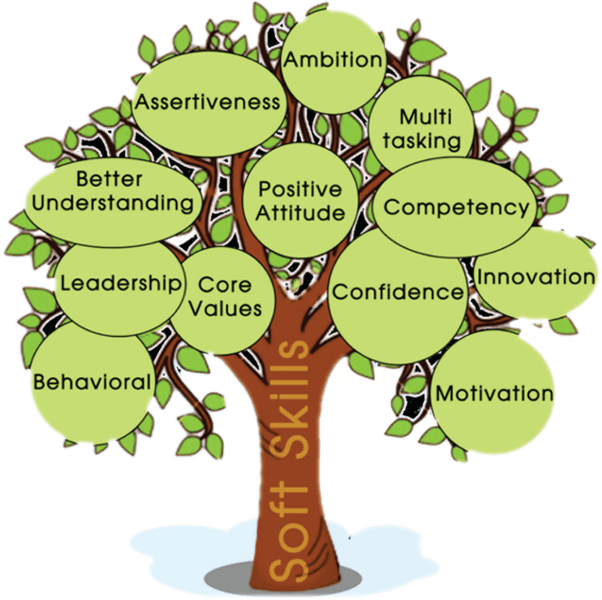
\includegraphics[width=1\linewidth]{soft_skills.png}
\caption{The Soft-Skills Tree}
\label{fig_sim}
\end{figure}

%%%%%%%%%%%%%%%%%%%%%%%%%%%%%%%%%%%%%%%%%%%%%%%%%%%%%%%%%%%%%%%%%%%%%%%%%%%%%%%%

\section{Future Work}

%%%%%%%%%%%%%%%%%%%%%%%%%%%%%%%%%%%%%%%%%%%%%%%%%%%%%%%%%%%%%%%%%%%%%%%%%%%%%%%%
\section{\IfLanguageName{english}{Conclusion}{Conclusão}}
The conclusions. Lorem ipsum dolor sit amet, consectetur adipiscing elit. Cras sed sapien quam. Sed dapibus est id enim facilisis, at posuere turpis adipiscing. Quisque sit amet dui dui.

Duis rhoncus velit nec est condimentum feugiat. Donec aliquam augue nec gravida lobortis. Nunc arcu mi, pretium quis dolor id, iaculis euismod ligula. Donec tincidunt gravida lacus eget lacinia. Lorem ipsum dolor sit amet, consectetur adipiscing elit.
%%%%%%%%%%%%%%%%%%%%%%%%%%%%%%%%%%%%%%%%%%%%%%%%%%%%%%%%%%%%%%%%%%%%%%%%%%%%%%%%
% references section
\bibliographystyle{IEEEtran}
%\bibliography{PP_Report_bib}
\bibliography{Mendeley}
%%%%%%%%%%%%%%%%%%%%%%%%%%%%%%%%%%%%%%%%%%%%%%%%%%%%%%%%%%%%%%%%%%%%%%%%%%%%%%%%
% biography section
% 
\begin{IEEEbiography}[{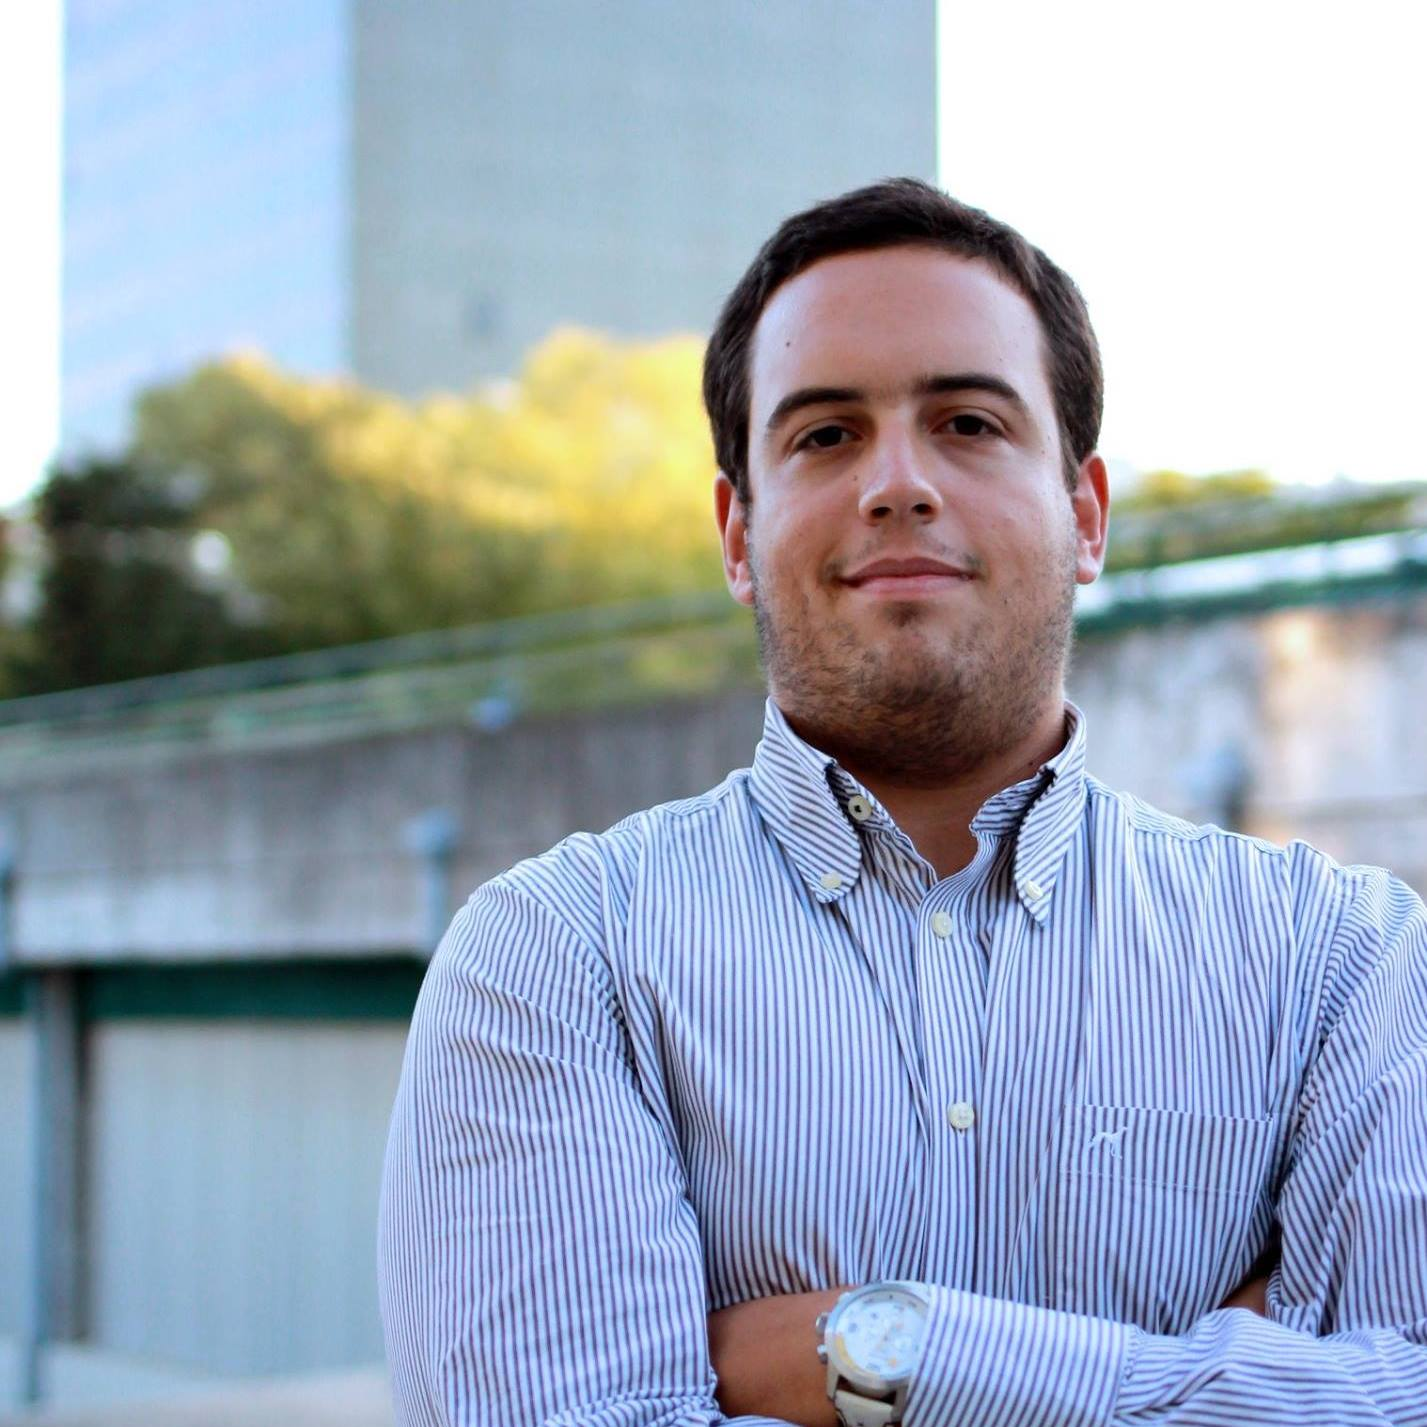
\includegraphics[width=1in,height=1.25in,clip,keepaspectratio]{bruno.png}}]{Bruno Cardoso}
Here I am. I am pursuing my Engineering studies at \ac{IST}. Starting my masters in Interaction and Visualization, and also on business systems. On my "spare" time, I am also developing a project at INESC-ID, at VIMMI.
\end{IEEEbiography}
\begin{IEEEbiography}
[{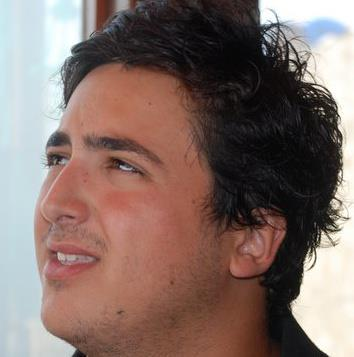
\includegraphics[width=1in,height=1.25in,clip,keepaspectratio]{francisco.png}}]{Francisco Maria Calisto}
I am pursuing my Information Systems and Computer  Engineering studies at \ac{IST}. I am also a VIMMI collaborator at INESC-ID. Currently I am working in a StartUp project called Agroop and I am Founder \& Front-end Developer of opprDev a oppr Group organisation.
\end{IEEEbiography}
\begin{IEEEbiography}
[{
\includegraphics[width=1in,height=1.25in,clip,keepaspectratio]{me.png}}]{Nuno Sousa}
Here I am. I am pursuing my Engineering studies at \ac{IST}. Lorem ipsum dolor sit amet, consectetur adipiscing elit. Cras sed sapien quam. Sed dapibus est id enim facilisis, at posuere turpis adipiscing. Quisque sit amet dui dui.Lorem ipsum dolor sit amet, consectetur adipiscing elit. 
\end{IEEEbiography}
%%%%%%%%%%%%%%%%%%%%%%%%%%%%%%%%%%%%%%%%%%%%%%%%%%%%%%%%%%%%%%%%%%%%%%%%%%%%%%%%
\newpage
\onecolumn
%%%%%%%%%%%%%%%%%%%%%%%%%%%%%%%%%%%%%%%%%%%%%%%%%%%%%%%%%%%%%%%%%%%%%%%%%%%%%%%%

%%%%%%%%%%%%%%%%%%%%%%%%%%%%%%%%%%%%%%%%%%%%%%%%%%%%%%%%%%%%%%%%%%%%%%%%%%%%%%%%
% *** DEFINITION OF ACRONYMS ***
	\acrodef{CPU}{Central Processing Unit}
	\acrodef{GUI}{Graphical User Interface}
	\acrodef{HTTP}{Hypertext Transfer Protocol}
	\acrodef{IST}{Instituto Superior Técnico}
	\acrodef{INESC-ID}{Instituto de Engenharia de Sistemas e Computadores - Investigação e Desenvolvimento}
	\acrodef{VIMMI}{Visualization and Intelligent Multimodal Interfaces}
	\acrodef{LAN}{Local Area Network}
	\acrodef{PC}{Personal Computer}
	\acrodef{URL}{Uniform Resource Locator}
	\acrodef{VoD}{Video-on-demand}
	\acrodefplural{VoD}[VoDs]{Videos-on-demand}
	\acrodef{VoIP}{Voice over IP}
	\acrodef{WAN}{Wide Area Network}
	\acrodef{WLAN}{Wireless Local Area Network}
	\acrodef{WWAN}{Wireless Wide Area Network}
	\acrodef{WWW}{World Wide Web}
	
% that's all folks
\end{document}